% Created 2018-12-02 Sun 18:24
% Intended LaTeX compiler: pdflatex
\documentclass[presentation]{beamer}
\usepackage[utf8]{inputenc}
\usepackage[T1]{fontenc}
\usepackage{graphicx}
\usepackage{grffile}
\usepackage{longtable}
\usepackage{wrapfig}
\usepackage{rotating}
\usepackage[normalem]{ulem}
\usepackage{amsmath}
\usepackage{textcomp}
\usepackage{amssymb}
\usepackage{capt-of}
\usepackage{natbib}
\usepackage[linktocpage,pdfstartview=FitH,colorlinks,
linkcolor=blue,anchorcolor=blue,
citecolor=blue,filecolor=blue,menucolor=blue,urlcolor=blue]{hyperref}
\setbeamertemplate{frame footer}{\insertshortauthor}
\setbeamerfont{page number in head/foot}{size=\tiny}
\setbeamercolor{footline}{fg=gray}
\usepackage{amsmath}
\author{Florian Hollenbach}
\usepackage[english]{isodate}
\usepackage{amsmath,amsthm,amssymb,amsfonts}
\newcommand{\E}{\mathbb{E}}
\newcommand{\V}{\mathbb{V}}
\usetheme{metropolis}
\usecolortheme{}
\usefonttheme{}
\useinnertheme{}
\useoutertheme{}
\author{Florian Hollenbach}
\date{\today}
\title{Political Science 209 - Fall 2018}
\subtitle{Uncertainty}

\hypersetup{
 pdfauthor={Florian Hollenbach},
 pdftitle={Political Science 209 - Fall 2018},
 pdfkeywords={},
 pdfsubject={},
 pdfcreator={Emacs 25.3.1 (Org mode 9.1.14)}, 
 pdflang={English}}
\begin{document}

\maketitle


\begin{frame}[label={sec:org8e0287a}]{Statistical Inference}
Goal: trying to estimate something unobservable from observable data

What we want to estimate: \alert{parameter} \(\theta\) \(\rightsquigarrow\) unobservable

What you do observe: \alert{data}

\pause

We use data to compute an estimate of the parameter \(\hat\theta\)
\end{frame}


\begin{frame}[label={sec:org949c286}]{Parameters and Estimators}
\begin{itemize}
\item \alert{parameter}: the quantity that we are interested in
\end{itemize}

\pause

\begin{itemize}
\item \alert{estimator}: method to compute parameter of interest
\end{itemize}
\end{frame}

\begin{frame}[label={sec:org24daec7}]{Parameters and Estimators}
Example:

\begin{itemize}
\item \alert{parameter}: support for Jimbo Fisher in student population

\item \alert{estimator}: sample proportion of support as estimator
\end{itemize}
\end{frame}

\begin{frame}[label={sec:orga2ced6c}]{Parameters and Estimators}
Example:

\begin{itemize}
\item \alert{parameter}: average causal effect of aspirin on headache

\item \alert{estimator}: difference in mean between treatment and control
\end{itemize}
\end{frame}


\begin{frame}[label={sec:org62b0cdf}]{Quality of estimators}
For the rest of the semester the question becomes:

\alert{How good is our estimator?}

\pause

\begin{enumerate}
\item \alert{How close in expectation is the estimator to the truth?}

\item \alert{How certain or uncertain are we about the estimate?}
\end{enumerate}
\end{frame}

\begin{frame}[label={sec:org2b15114}]{Quality of estimators}
How good is \(\hat\theta\) as an estimate of \(\theta\)?

\begin{itemize}
\item Ideally, we want to know \alert{estimation error} \(= \hat\theta - \theta_{truth}\)
\end{itemize}

But we can never calculate this. Why?

\pause

\(\theta_{truth}\) is unknown

\emph{If we knew what the truth was, we didn't need an estimate}
\end{frame}

\begin{frame}[label={sec:orgf0164f2}]{Quality of estimators}
Instead, we consider two hypothetical scenarios:
\begin{enumerate}
\item How well would \(\hat\theta\) perform over \emph{repeated data generating processes}? (\alert{bias})
\item How well would \(\hat\theta\) perform as the sample size goes to infinity? (\alert{consistency})
\end{enumerate}
\end{frame}

\begin{frame}[label={sec:org5ec6191}]{Bias}
\begin{itemize}
\item Imagine the estimate being a random variable itself

\item Drawing infinitely many samples of students asking about Jimbo
\end{itemize}

What is the average of the sample average? Or what is the expectation of the estimator?

bias = \(\E\)(estimation error) = \(\E\)(estimate - truth) = \(\E(\bar{X})\) - p = p - p = 0
\end{frame}


\begin{frame}[label={sec:org76b841e}]{Bias - \alert{Important}}
\alert{An unbiased estimator does not mean that it is always exactly correct!}

\pause
\alert{To remember:} bias measures whether in expectation (on average) the estimator is giving us the truth
\end{frame}

\begin{frame}[label={sec:orgc11e171}]{Consistency}
Essentially saying that the law of large numbers applies to the estimator, i.e.:

\alert{An estimator is said to be consistent if it converges to the parameter (truth) if N goes to \(\infty\)}
\end{frame}


\begin{frame}[label={sec:orgd72da23}]{Variability}
Next, we have to consider how certain we are about our results

Consider two estimators:

\begin{enumerate}
\item slightly \emph{biased}, on average off by a bit, but always by the same margin

\item unbiased, but misses target left and right
\end{enumerate}
\end{frame}


\begin{frame}[label={sec:org1cf0db6}]{Variability}
\begin{center}
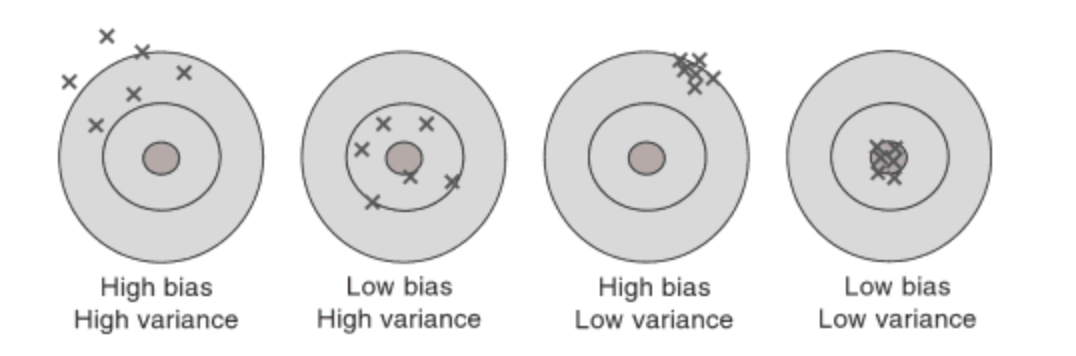
\includegraphics[width=6cm]{/Users/florianhollenbach/Documents/GitHub/Polisci209_2018/slides/week13/DART.png}
\end{center}

(Encyclopedia of Machine Learning)
\end{frame}

\begin{frame}[label={sec:org35842e3}]{Variability}
We characterize the variability of an estimator by using the standard deviation of the sampling distribution

\alert{How do we find that????}

\pause

Remember, the sampling distribution is the distribution of our statistic over hypothetical infinitely many samples
\end{frame}

\begin{frame}[label={sec:orgc0b6ce4}]{Variability}
\begin{center}
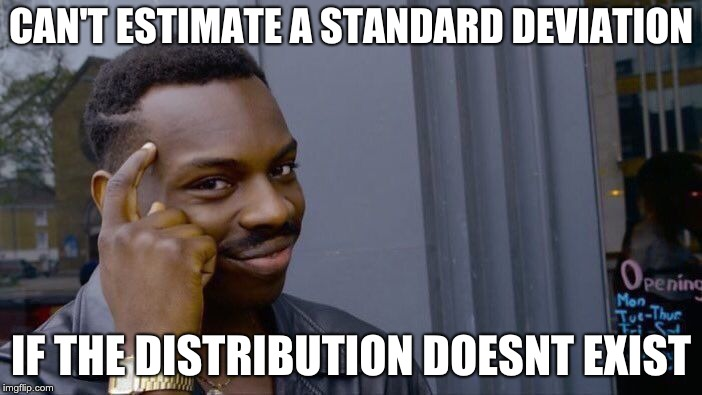
\includegraphics[width=6cm]{/Users/florianhollenbach/Documents/GitHub/Polisci209_2018/slides/week13/2mi1j5.jpg}
\end{center}
\end{frame}


\begin{frame}[label={sec:org4ae6e40}]{Standard Error}
We estimate the standard deviation of the sampling distribution from the observed data

\alert{standard error}

\pause

``\emph{standard error} and describes the (estimated) average degree to which an estimator deviates from its expected value'' (Imai 2017)
\end{frame}

\begin{frame}[label={sec:orgcda7680}]{Polling Example}
Say we took a sample of 1500 students and asked whether they support Jimbo or not

Define a random variable \(X_{i} = 1\) if student \emph{i} supports Jimbo, \(X_{i}=0\) if not

\pause

Binomial distribution with success probability p and size N where p is the proportion of \emph{all students} who support Jimbo (population dist)
\end{frame}


\begin{frame}[label={sec:org4e1e90d}]{Polling Example}
Estimator: ?
\end{frame}

\begin{frame}[label={sec:org8387c50}]{Polling Example}
Estimator: \(\overline{X} = \frac{1}{N} \sum_{i=1}^{N} X_{i}\)

\pause

In earlier notation: \(\theta_{truth} =p\) and \(\theta = \overline{X}\)
\end{frame}


\begin{frame}[label={sec:org3dbf3be}]{Polling Example}
Estimator: \(\overline{X} = \frac{1}{N} \sum_{i=1}^{N} X_{i}\)

\begin{enumerate}
\item LLN: \(\overline{X} \longrightarrow p\) (\alert{consistent})

\item Expectation: \(\E(\overline{X}) = p\) (\alert{unbiased})

\item standard error?
\end{enumerate}
\end{frame}


\begin{frame}[label={sec:org045e573}]{Polling Example - standard error}
\(X_i\) are i.i.d Bernoulli random variables with probability = p


\(\V(\overline{X}) = \frac{1}{N^{2}} \V(\sum_{i=1}^{N}X_{i})  = \frac{1}{N^{2}} \sum_{i=1}^{N} \V(X_{i})\)
\end{frame}


\begin{frame}[label={sec:org987a132}]{Polling Example - standard error}
\(X_i\) are i.i.d Bernoulli random variables with probability = p


\(\V(\overline{X}) = \frac{1}{N^{2}} \V(\sum_{i=1}^{N}X_{i})  = \frac{1}{N^{2}} \sum_{i=1}^{N} \V(X_{i}) = \frac{N}{N^{2}} \V(X)\)
\end{frame}


\begin{frame}[label={sec:org3f2eec5}]{Polling Example - standard error}
\(X_i\) are i.i.d Bernoulli random variables with probability = p


\(\V(\overline{X}) = \frac{1}{N^{2}} \V(\sum_{i=1}^{N}X_{i})  = \frac{1}{N^{2}} \sum_{i=1}^{N} \V(X_{i}) = \frac{N}{N^{2}} \V(X) = \frac{p \times (1-p)}{N}\)
\end{frame}

\begin{frame}[label={sec:org96767e9}]{Polling Example - standard error}
\(\V(\overline{X}) = \frac{p \times (1-p)}{N}\)

Standard error: \(\sqrt{\V(\overline{X})}\)

But we don't know p! Now what?

\pause

We use our unbiased estimate of p: \overline{X}
\end{frame}

\begin{frame}[label={sec:org1fa5a8a}]{Polling Example - standard error estimate}
\(\sqrt{\widehat{\V(\overline{X})}} = \sqrt{\frac{\overline{X}(1-\overline{X})}{N}}\)
\end{frame}

\begin{frame}[label={sec:org35aa5c0}]{Polling Example - standard error estimate}
Assume in our sample 55\% of students support Jimbo:

SE = \(\sqrt{\widehat{\V(\overline{X})}} = \sqrt{\frac{0.55 \times (1-0.55)}{1500}} = \sqrt{\frac{0.55 \times (0.45)}{1500}} = 0.013\)

We can expect our estimate on average to be off by 1.3 percentage points

\pause

If \(\overline{X}\) = 0.8, then SE = 0.010

If N = 500, \(\overline{X}\) = 0.55, then SE = 0.022
\end{frame}

\begin{frame}[label={sec:org88a634f}]{Standard error estimate}
Standard error is based on variance of the sampling distribution

Gives estimate of uncertainty

Each estimator/statistic has unique sampling distribution, e.g. difference in means
\end{frame}

\begin{frame}[label={sec:org506c89b}]{Confidence Intervals}
Often we don't even know the sampling distribution of our estimators

How could we approximate it?


\pause
\alert{Central limit theorem!}
\end{frame}


\begin{frame}[label={sec:org85a0fba}]{Confidence Intervals}
Central limit theorem says:

\(\overline{X} \approx N(\E(X), \frac{\V(X)}{N})\)

\alert{regardless of distribution of X}
\end{frame}


\begin{frame}[label={sec:orgce0e3f3}]{Confidence Intervals}
We can use the approximation to the sampling distribution, \(\overline{X} \approx N(\E(X), \frac{\V(X)}{N})\) to construct \alert{confidence intervals}

Confidence intervals give a range of values that is likely to contain the true value

\pause
To start, we select a probability value for our confidence level: usually 95\%
\end{frame}

\begin{frame}[label={sec:org58d39e8}]{Confidence Intervals}
\alert{The 95\% confidence interval specifies the range of values in which the true parameter will fall for 95\% of our hypothetical samples/experiments}

\pause

Put differently
\alert{``Over a hypothetically repeated data generating process, confidence intervals contain the true value of parameter with the probability specified by the confidence level''} (Imai 2017)
\end{frame}


\begin{frame}[label={sec:org3220d12}]{Confidence interval}
(1-\(\alpha\)) large sample Confidence interval is defined as:

CI(\(\alpha\)) = \(\overline{X} - z_{\frac{\alpha}{2}} \times SE\),  \(\overline{X} + z_{\frac{\alpha}{2}} \times SE\)

\(z_{\frac{\alpha}{2}}\) is the critical value which equals (1 − \(\frac{\alpha}{2})\) quantile of the standard normal distribution
\end{frame}

\begin{frame}[label={sec:org31d97a9}]{Confidence interval}
Where do the critical values come from?

\pause
Remember: Curve of the standard normal distribution:

\begin{itemize}
\item Symmetric around 0
\item Total area under the curve is 100\%
\item Area between -1 and 1 is \textasciitilde{}68\%
\item Area between -2 and 2 is \textasciitilde{}95\%
\item Area between -3 and 3 is \textasciitilde{}99.7\%
\end{itemize}
\end{frame}

\begin{frame}[label={sec:org08ebed9}]{Confidence interval}
\begin{center}
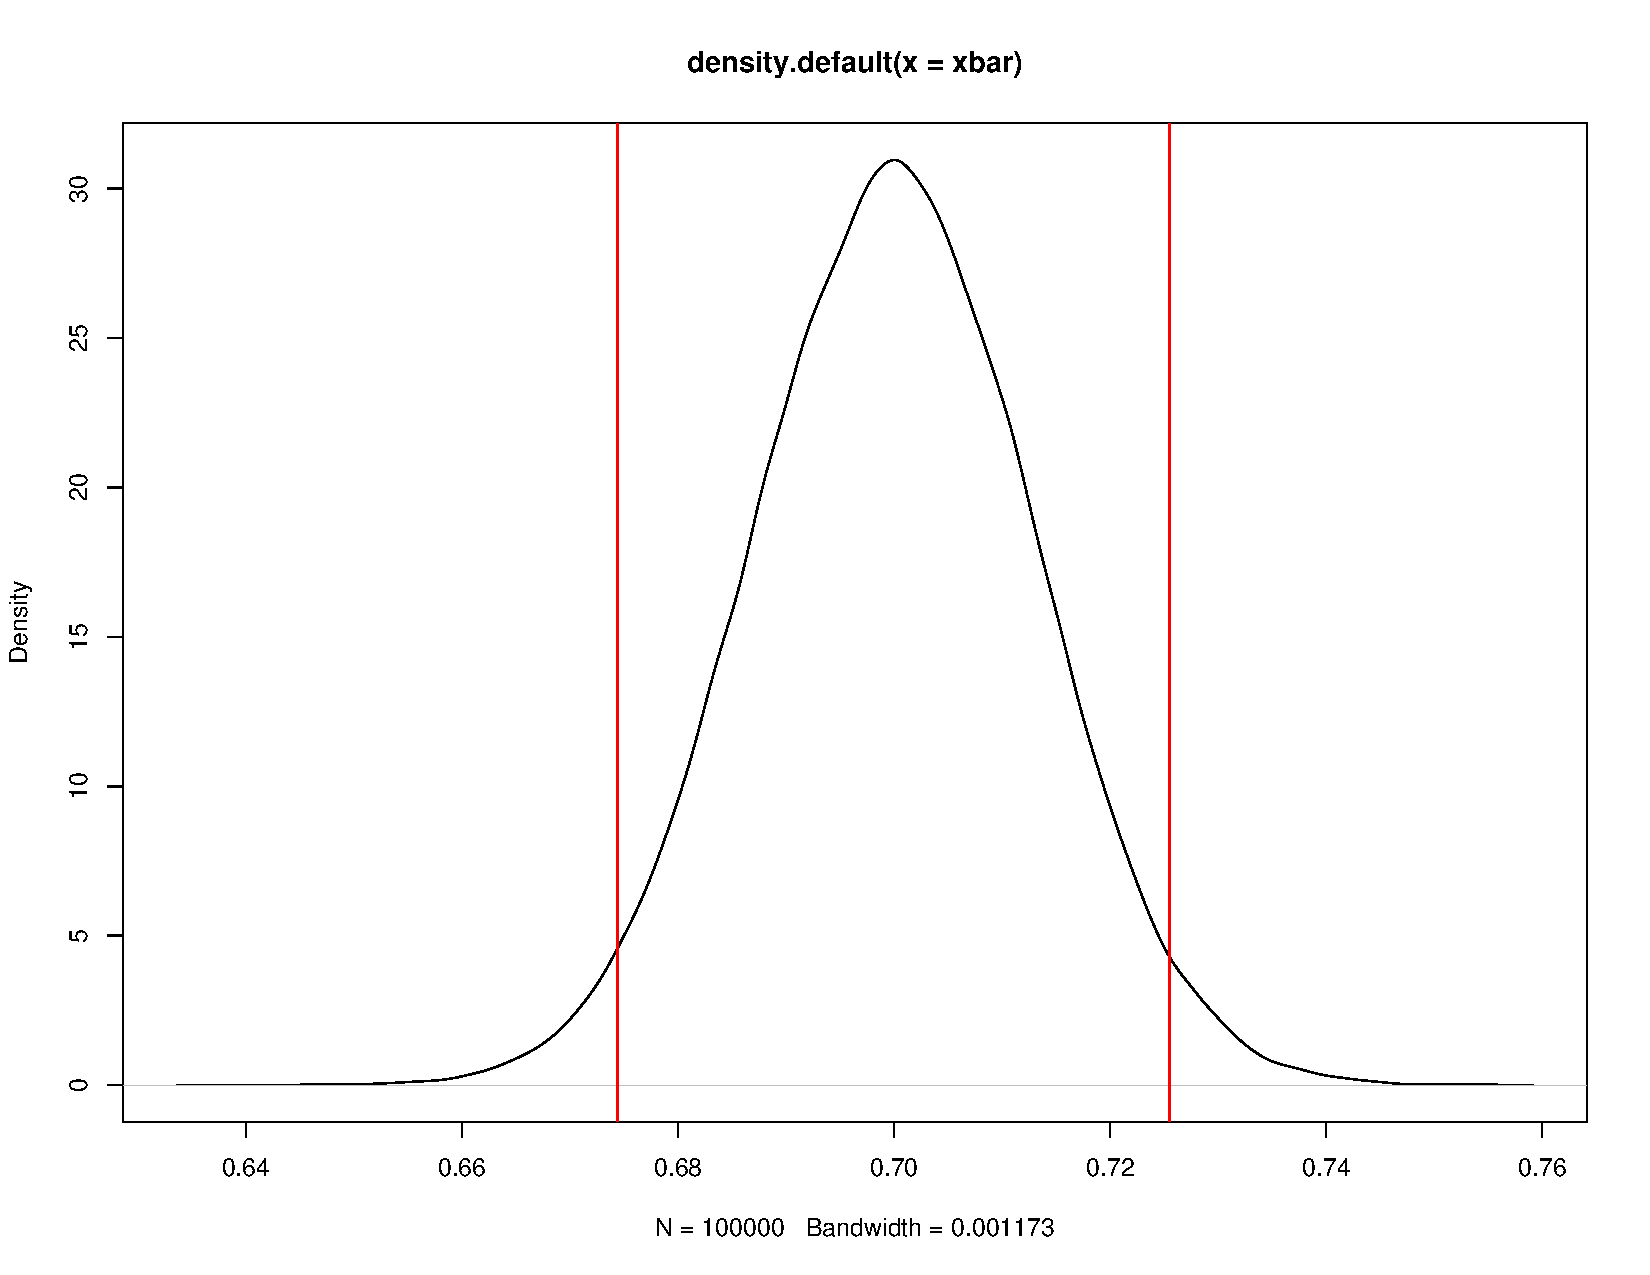
\includegraphics[width=6cm]{/Users/florianhollenbach/Documents/GitHub/Polisci209_2018/slides/week13/Norm_density.pdf}
\end{center}

\alert{Critical values are the exact vales between which the standard normal distribution will include (1-\(\alpha\)) \% of the area}
\end{frame}

\begin{frame}[label={sec:org89bc07c}]{Confidence interval interpretation}
Technically the CI is \alert{not} the probability of the true parameter being between the two value.

\pause
Remember, in our view the true parameter is fixed

Instead: ``95\% confidence intervals contain the true value of the parameter 95\% of the time during a hypothetically repeated data generating process'' (Imai 2017)
\end{frame}

\begin{frame}[label={sec:org91b212d}]{Confidence interval interpretation}
Remember in the Jimbo example with \(\overline{X} = 0.55\) and N = 1500

SE = \(\sqrt{\widehat{\V(\overline{X})}} = \sqrt{\frac{0.55 \times (1-0.55)}{1500}} = \sqrt{\frac{0.55 \times (0.45)}{1500}} = 0.013\)
\end{frame}

\begin{frame}[label={sec:org2db94b3}]{Confidence interval}
CI(\(\alpha\)) = \(\overline{X} - z_{\frac{\alpha}{2}} \times SE\),  \(\overline{X} + z_{\frac{\alpha}{2}} \times SE\)

\pause

CI(0.05) = \(0.55 - 1.96 \times 0.013\),  \(0.55 +  1.96 \times 0.013\) = 0.524, 0.576
\end{frame}


\begin{frame}[fragile,label={sec:org6f5c86f}]{Confidence interval}
 What if we don't know the variance of the estimator?

Let's use the variance of the sample?

\begin{verbatim}
x <- rbinom(1500,1,0.7)
var <-var(x)/1500
SE <- sqrt(var)
\end{verbatim}

SE = 0.013
\end{frame}


\begin{frame}[fragile,label={sec:org1149f61}]{Confidence interval}
 \begin{verbatim}
xbar <- rep(NA, 10000)
for(i in 1:10000){
  x <- rbinom(1500,1,0.55)
  xbar[i] <-mean(x)
}
\end{verbatim}

Write an R-script to test our confidence interval for Jimbo!
\end{frame}


\begin{frame}[label={sec:orgcc7d6be}]{Margin of Error in Surveys}
\begin{itemize}
\item Margin of error is usually the difference from estimate to upper/lower 95$\backslash$% confidence interval

\item Margin of error: \(z_{0.025} \times \hat{SE} \approx  z_{0.025} \times \sqrt{\frac{\overline{X} \times (1-\overline{X})}{N}}\)
\end{itemize}
\end{frame}


\begin{frame}[label={sec:orgac89161}]{From Margin of Error to Sample Size}
N \(\approx \frac{1.96 \times p \times (1-p)}{\text{margin of error}^{2}}\)
\end{frame}


\begin{frame}[label={sec:orgb9206e4}]{From Margin of Error to Sample Size}
The estimates of uncertainty discussed here only account for uncertainty due to random sampling!

If there are other sources of bias, these can still be present and are unaccounted for.

\alert{what are two possibly reasons for bias in surveys?}

\pause

\begin{enumerate}
\item unit non-response bias
\item item non-response bias
\end{enumerate}
\end{frame}

\begin{frame}[label={sec:orga2ca7c4}]{Uncertainty in Randomized Control Trials}
How do we estimate the ATE in RTCs?

\pause

Difference in means between treatment and control group
\end{frame}

\begin{frame}[label={sec:orgb035aa6}]{Uncertainty in Randomized Control Trials}
sample average in treated group \(\overline{X}_{c}\) and control group \(\overline{X}_{c}\)

\pause


Standard error for the average in each group:
\begin{enumerate}
\item \(\hat{SE}_{t} = \sqrt{\frac{\hat{\sigma}^{2}_{t}}{N_{t}}}\)
\item \(\hat{SE}_{c} = \sqrt{\frac{\hat{\sigma}^{2}_{c}}{N_{c}}}\)
\end{enumerate}

What do we use for \(\hat{\sigma^{2}}\)?
\pause
sample variance! \(\frac{\sum (\overline{X} - X_{i})^{2}}{N}\)
\end{frame}

\begin{frame}[label={sec:org3b65bd1}]{Uncertainty in Randomized Control Trials}
We can use these SEs to construct confidence intervals around each of the averages, same process as for the survey (\alert{if the samples are large enough})

But, this does not help us to calculate uncertainty for the difference in means.
\end{frame}


\begin{frame}[label={sec:org26fb154}]{Uncertainty in Randomized Control Trials}
Standard Error for difference in means estimator (\(\overline{X}_{t} - \overline{X}_{c}\)):

\(\hat{SE} = \sqrt{\frac{\V(X_{t})}{N_{t}} + \frac{\V(X_{c})}{N_{c}}}\)
\end{frame}

\begin{frame}[label={sec:org6ba0ec5}]{Uncertainty in Randomized Control Trials}
We can use the standard error to construct a 95\% confidence interval for the difference in means:

Example: ATE = 3.5, SE = 2.65

CI?
\end{frame}

\begin{frame}[label={sec:orge3e0e80}]{Uncertainty in Randomized Control Trials}
We can use the standard error to construct a 95\% confidence interval for the difference in means:

Example: ATE = 3.5, SE = 2.65

CI(0.05) = \(3.5 - 1.96 \times 2.65\),  \(3.5 +  1.96 \times 2.65\) = -1,694, 8.694

\alert{Too much uncertainty}
\end{frame}


\begin{frame}[label={sec:org009b2df}]{Uncertainty in Randomized Control Trials}
When evaluating effects, we usually judge them based on whether the 95\% confidence interval covers zero or not.
\end{frame}


\begin{frame}[shrink=25,label={sec:org03d5b43}]{In class Exercise}
To isolate the causal effect of a criminal record for black and white applicants, Pager ran an audit experiment. In this type of experiment, researchers present two similar people that differ only according to one trait thought to be the source of discrimination.

To examine the role of a criminal record, Pager hired a pair of white men and a pair of black men and instructed them to apply for existing entry-level jobs in the city of Milwaukee. The men in each pair were matched on a number of dimensions, including physical appearance and self-presentation. As much as possible, the only difference between the two was that Pager randomly varied which individual in the pair would indicate to potential employers that he had a criminal record. Further, each week, the pair alternated which applicant would present himself as an ex-felon. To determine how incarceration and race influence employment chances, she compared callback rates among applicants with and without a criminal background and calculated how those callback rates varied by race.
\end{frame}

\begin{frame}[label={sec:orgc80bb60}]{In class Exercise}
Download data criminalrecord.csv from the class website and read into \emph{R}

Summarize the data, what variables do you see?
\end{frame}


\begin{frame}[shrink=30,label={sec:org31716a0}]{In class Exercise}
\begin{center}
\begin{tabular}{ll}
Name & Description\\
jobid & Job ID number\\
callback & 1 if tester received a callback, 0 if the tester did not receive a callback.\\
black & 1 if the tester is black, 0 if the tester is white.\\
crimrec & 1 if the tester has a criminal record, 0 if the tester does not.\\
interact & 1 if tester interacted with employer during application, 0 if tester doesn’t\\
city & 1 is job is located in the city center, 0 if job is located in the suburbs.\\
distance & Job’s average distance to downtown.\\
custserv & 1 if job is in the costumer service sector, 0 if it is not.\\
manualskill & 1 if job requires manual skills, 0 if it does not.\\
\end{tabular}
\end{center}
\end{frame}


\begin{frame}[label={sec:orgd927e0b}]{Question 1}
How many observations are in the data? In how many cases is the tester black? In how many cases is he white?
\end{frame}

\begin{frame}[label={sec:org120f30f}]{Question 2}
Now we examine the central question of the study. Calculate the proportion of callbacks for white applicants with a criminal record, white applicants without a criminal record, black applicants with a criminal record, and black applicants without a criminal record.
\end{frame}

\begin{frame}[label={sec:org73885d6}]{Question 3}
Now consider the callback rate for white applicants with a criminal record. Construct a 95\% confidence interval around this estimate. Also, construct a 99\% confidence interval around this estimate.
\end{frame}

\begin{frame}[label={sec:orge779d42}]{Question 4}
Calculate the estimated effect of a criminal record for white applicants by comparing the callback rate in the treatment condition and the callback rate in the control condition. Create a 95\% confidence interval around this estimate. Next, describe the estimate and confidence interval in a way that could be understood by a general audience.
\end{frame}

\begin{frame}[label={sec:orgd95c8b3}]{Question 5}
Assuming a null hypothesis that there is no difference in callback rates between white people with a criminal record and white people without a criminal record, what is the probability that we would observe a difference as large or larger than the one that we observed in a sample of this size?
\end{frame}
\end{document}